\documentclass[../main.tex]{subfiles}
\begin{document}
\setchapterstyle{kao}
\setchapterpreamble[u]{\margintoc}
\chapter[Lie groups II - important examples]{Lie groups II - important examples\footnotemark[0]}
\labch{Lie-groups-II}
\section{Generalized orthogonal groups O(p,q) (including the \href{https://it.wikipedia.org/wiki/Hendrik_Lorentz}{Lorentz} group O(1,3))}
\labsec{GOG}
As we have seen in the review of relativistic mechanics [\refsec{RMReview}], the Lorentz metric has signature (1,3) so when diagonalized it has one positive eigenvalues and three negative ones. We can generalize this concept and have $p$ positive eigenvalues and $q$ negative ones: the properties of the group will change depending on $p$ and $q$. We fix $p,q\in\mathbb{N}^x$ which will be the signature of our metric, we set $V\cong\mathbb{R}^{p+q}$ and define:\marginnote{One could use the Lorentz metric with signature (3,1) and have three positive eigenvalues and a negative one, depending on the convention used.}
% \[
% \begin{pNiceMatrix}[first-row,first-col]
% & & \Ldots[line-style={solid,<->}]^{n \text{ columns}} \\
% & 1 & 1 & 1 & \Ldots & 1 \\
% & 1 & 1 & 1 & & 1 \\
% \Vdots[line-style={solid,<->}]_{n \text{ rows}} & 1 & 1 & 1 & & 1 \\
% & 1 & 1 & 1 & & 1 \\
% & 1 & 1 & 1 & \Ldots & 1
% \end{pNiceMatrix}
% \]
\[
G=g_{ij}=
\left(\begin{array}{cccc:ccc}
    +1&&& & 0&0&0 \\
    &+1&& & 0&0&0 \\
    &&+1& & 0&0&0 \\
    &&&+1 & 0&0&0 \\
    \hdashline
    0&0&0&0 & -1&&\\ 
    0&0&0&0 & &-1& \\
    0&0&0&0 & &&-1 \\
\end{array}\right)
% \begin{pNiceArray}{cccc|ccc}[margin]
% 1&&& & 0&0&0\\ 
% %\Vdotsfor[line-style={solid,<->,xshift=8mm}]{4}^{\rotatebox{90}{p}}\\
% &1&& & 0&0&0 \\
% &&1& & 0&0&0 \\
% &&&1 & 0&0&0 \\
% \hline
% 0&0&0&0 & -1&&\\ %\Vdotsfor[line-style=V]{3}^{\rotatebox{90}{q}}\\
% 0&0&0&0 & &-1& \\
% 0&0&0&0 & &&-1 \\
% % \Hdotsfor[line-style=H]{4}^{\rotatebox{0}{p}} & \Hdotsfor[line-style=H]{3}^{\rotatebox{0}{q}}
% \end{pNiceArray}
\marginnote{This is a $(p+q)\times(p+q)$ matrix.}
\]
\begin{marginfigure}[-10mm]
	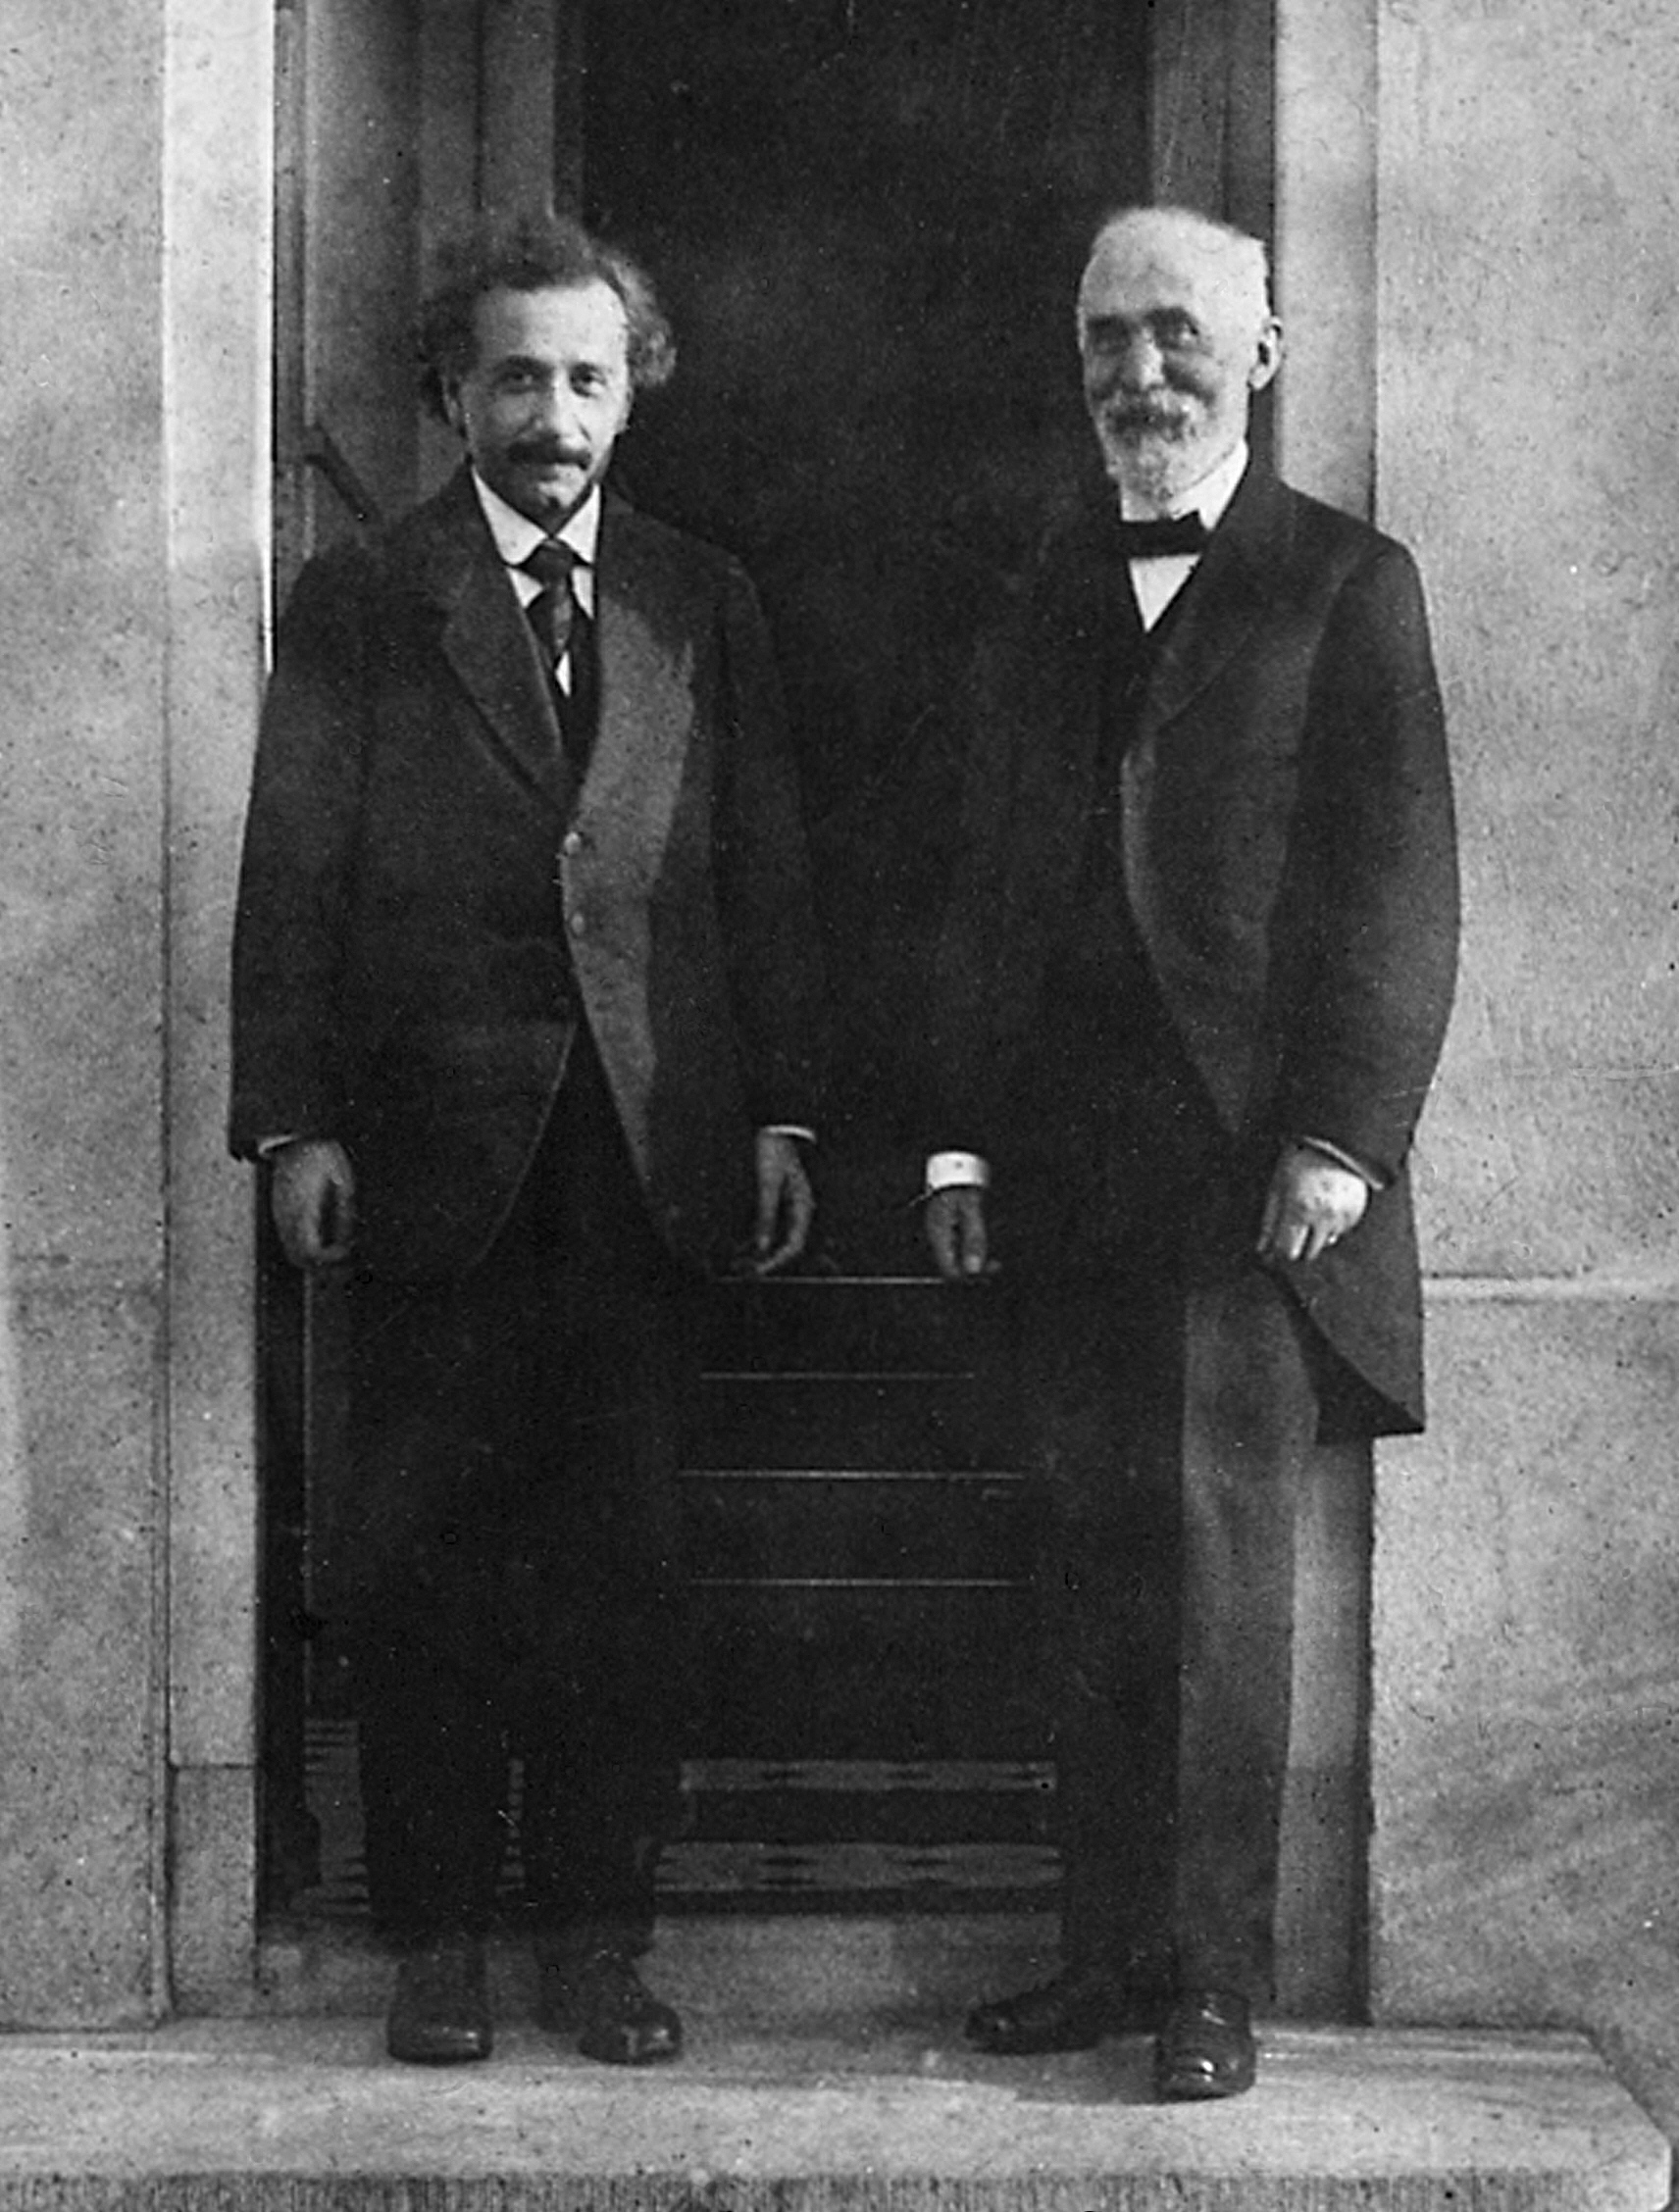
\includegraphics[width=1\linewidth]{images/Einstein_en_Lorentz.jpg}
	\caption[Photo of Albert Einstein and Hendrik Antoon Lorentz]{From \href{https://commons.wikimedia.org/wiki/File:Einstein_en_Lorentz.jpg}{Wikimedia}: Albert Einstein and Hendrik Antoon Lorentz, photographed by Paul Ehrenfest (1880-1933) in front of his home in Leiden in 1921.}
	\labfig{Lorentz}
\end{marginfigure}
With the help of that, we define a map:
\begin{align*}
\langle\dots,\dots\rangle_G: V\times V &\xrightarrow[]{}\mathbb{R}\\
(v,w) &\mapsto\langle v,w\rangle_G
\end{align*}
defined by \({\color{red} \langle v,w \rangle_G} {\color{red}=\sum_{i,j=1}^n g_{ij}v^iw^j}\). For $(p,q)=(n,0)$ we recover the \textbf{Euclidean case}, for $(p,q)=(1,3)$ we recover the \textbf{Lorentzian case.}%37:00
\begin{definition}[G-orthogonal]\index{G-orthogonal}
We say that $A\in \textrm{End}(\mathbb{R}^{p+q})$ is \textbf{G-orthogonal}\footnote{or orthogonal with respect to the matrix $G$} if it happens that $({{A}}v,{{A}}w)_G=(v,w)_G \; \forall v,w\in V$.
\end{definition}
\begin{definition}[Generalized orthogonal group]\index{Generalized orthogonal group}
The \textbf{generalized orthogonal group} $\textrm{O}(p,q)$ is defined as:
\[
\textrm{O}(p,q)=\Bqty{A\in \textrm{End}(\mathbb{R}^{p+q}):\ A \textrm{ is \textbf{G-orthogonal}}}
\]
\end{definition}
\todo{Now set $q=0$}
One checks $\textrm{O}(p,0)\subseteq GL(\mathbb{R}^p)$. Take $A\in O(p,0)$:
\[
\text{Ker}A=\{v\in V:||Av||_G^2=0\}\underset{\mathclap{\tikz \node {$\uparrow$} node [below=1ex] {\footnotesize A is \textbf{G-orthogonal} };}}=\{v\in V:||v||_G^2=0\}\underset{\mathclap{\tikz \node {$\uparrow$} node [below=1ex] {\footnotesize only for $(p,0)$ or $(q,0)$ };}}=\{0\}
\]
Therefore, $A$ is \textbf{injective}. Since $\text{dim}V<+\infty$, then it is also \textbf{surjective}, therefore it is a bijection and hence invertible.
\begin{starredExercise}:
\begin{enumerate}
    \item Prove that $A\in \textrm{O}(p,q)$ if and only if {\color{red}$A^TGA=G$}\marginnote{If $G=\mathbb{1}$, i.e. the Euclidean case, we recover that $A^TA=\mathbb{1}$.}
    \item Use 1) to prove that $\textrm{O}(p,q)$ is a \textbf{closed subgroup} of $\textrm{GL}(\mathbb{R}^{p+q})$, hence a \textbf{Lie subgroup} (use Cartan's criterion).
\end{enumerate}
\end{starredExercise}
\section{Symplectic groups}
Let $V\cong\mathbb{R}^{\color{red}2n}$ (\textbf{even dimensions!}). We define $\Omega=\left(\begin{array}{c:c}
    0 & +\mathbb{1} \\
    \hdashline
    -\mathbb{1} & 0
\end{array}\right)$ and introduce $\omega$:
\begin{equation}\labeq{sympl-bil-form}
\begin{split}
    \omega: V\times V &\xrightarrow[]{}\mathbb{R}\\
    (v,w) &\mapsto \omega(v,w)
    \end{split}
\end{equation}
by setting ${\color{red}\omega(v,w)}{\color{red}=\sum_{i,j=1}^n\Omega_{ij}v^iw^j}$. Then $\omega$ is \textbf{bilinear}, \textbf{anti-symmetric} and \textbf{non-degenerate}:
\[
\textrm{if }\ \Big(\omega(v,w)=0 \; \forall \ w \in V\Big)\quad \Rightarrow v=0
\]
\begin{marginfigure}
	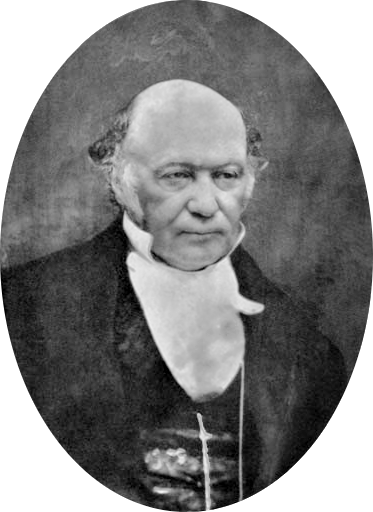
\includegraphics[width=1\linewidth]{images/William_Rowan_Hamilton_portrait_oval_combined.png}
	\caption[Sir William Rowan Hamilton.]{From \href{https://commons.wikimedia.org/wiki/File:William_Rowan_Hamilton_portrait_oval_combined.png}{Wikimedia}: Sir William Rowan Hamilton LL.D, DCL, MRIA, FRAS (3/4 August 1805 – 2 September 1865) was an Irish mathematician, Andrews Professor of Astronomy at Trinity College Dublin, and Royal Astronomer of Ireland at Dunsink Observatory. He made major contributions to optics, classical mechanics and abstract algebra. His work was of importance to theoretical physics, particularly his reformulation of Newtonian mechanics, now called Hamiltonian mechanics. It is now central both to electromagnetism and to quantum mechanics. In pure mathematics, he is best known as the inventor of quaternions. Hamilton retained his faculties unimpaired to the last, and continued the task of finishing the Elements of Quaternions which had occupied the last six years of his life. He died on 2 September 1865, following a severe attack of gout. He is buried in Mount Jerome Cemetery in Dublin.}
	\labfig{SirHamilton}
\end{marginfigure}
\underline{\textbf{Motivation:}} We take $\mathbb{R}^{2n}=(q,p)$. We write down Hamilton equations (without following precisely the Ricci's indices):
\begin{equation}\labeq{ham-eq}
\begin{pmatrix}
\Dot{q}\\
\Dot{p}
\end{pmatrix}
=
\left(
\begin{array}{c:c}
    0 & +\mathbb{1} \\
    \hdashline
    -\mathbb{1} & 0
\end{array}
\right)
\begin{pmatrix}
\frac{\partial\pazocal{H}}{\partial q^j}\\
\cdots\\
\frac{\partial\pazocal{H}}{\partial p^j}
\end{pmatrix}
\end{equation}
So we can rewrite Hamilton's equation by involving this $\omega^{-1}$ matrix (in this case $=\omega$). Hamiltonian dynamical systems have a lot of nice properties (conservation of energy, conservation of volume in phase space, existence of the solution at every time etc...) and are very nice mathematical objects, so people ask themselves how much these nice properties depend on the fact that the matrix has exactly the structure which is written here in \refeq{ham-eq}. The answer is that they do not depend so much, in the sense that they depend on the fact that this matrix induces a bilinear form $\omega$ in \refeq{sympl-bil-form} which is bilinear, anti-symmetric and non degenerate. Therefore if we change $\omega$ a little bit, by putting a term of order $\pazocal{O}(\varepsilon)$ in the upper left block of $\Omega$, this would still induce a bilinear $\omega$, also anti-symmetric (if you are careful that the piece of order $\varepsilon$ is anti-symmetric) and still non degenerate, because before the perturbation the determinant was $1$, and after the perturbation it will be of order $1+\pazocal{O}(\varepsilon)\neq 0$ (for $\varepsilon$ sufficiently small). This field of research is called \textit{Symplectic geometry}, namely the geometry behind the hamiltonian systems and their generalizations.

Let us emphasize that we are taught in every course that the Hamiltonian formulation is not so nice, because it is not relativistic covariant. This is definitely true, to talk about some relativistic phenomenon is better to have a Lagrangian formulation of our dynamical theory, nevertheless it has many other advantages in any other context (non-relativist ones). For example Liouville theorem (conservation of volume space) is a property of generalized Hamiltonian systems which depends only on the fact that $\omega$ has the previous properties.

Now we want the group of transformations which are, in a sense, orthogonal with respect to this bilinear form. This is something much different from the previous case, because now $\omega$ is not an inner product (a scalar product), but it is anti-symmetric.
\begin{definition}[Real symplectic group]\index{Real symplectic group}
The \textbf{real symplectic group} $S_P(n,\mathbb{R})$ is defined as the set of $A\in \textrm{End}(\mathbb{R}^{{2n}})$ such that 
\[
\omega({A}v,{A}w)=\omega(v,w)\quad\forall\; v,w\in V
\]
\end{definition}
\begin{exercise}:\marginnote{You can exchange the previous starred exercise with this one, but not do both.}
\begin{enumerate}
    \item $A\in \text{S}_\text{P}(n,\mathbb{R})$ if and only if ${\color{red}-\Omega A^T\Omega=A^{-1}}$
    \item Use 1) to prove that $\text{S}_\text{P}(n,\mathbb{R})$ is a \textbf{Lie subgroup} of $\textrm{GL}(\mathbb{R}^{2n})$
\end{enumerate}
\end{exercise}
\section{Euclidean and Poincaré group}
\labsec{Euclidean-and-Poincaré-group}
\begin{marginfigure}
	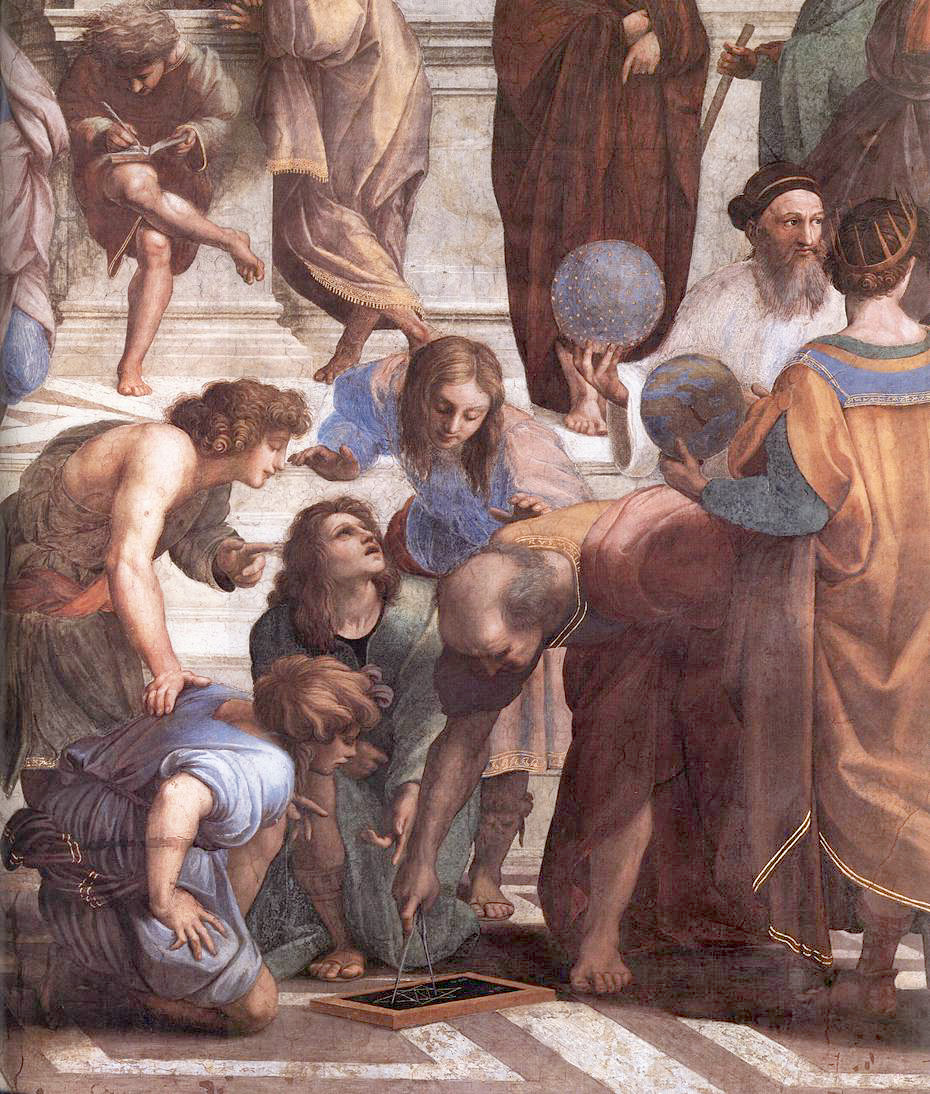
\includegraphics[width=1\linewidth]{images/Sanzio_01_Euclid.jpg}
	\caption[Detail from Raphael's The School of Athens presumed to represent Donato Bramante as Euclid.]{From \href{https://commons.wikimedia.org/wiki/File:Sanzio_01_Euclid.jpg}{Wikimedia}: Detail from Raphael's The School of Athens presumed to represent Donato Bramante as Euclid. Euclid (Greek: Eukleides; fl. 300 BC), sometimes called Euclid of Alexandria to distinguish him from Euclid of Megara, was a Greek mathematician, often referred to as the "founder of geometry" or the "father of geometry". He was active in Alexandria during the reign of Ptolemy I (323–283 BC). His Elements is one of the most influential works in the history of mathematics, serving as the main textbook for teaching mathematics (especially geometry) from the time of its publication until the late 19th or early 20th century. In the Elements, Euclid deduced the theorems of what is now called Euclidean geometry from a small set of axioms. Euclid also wrote works on perspective, conic sections, spherical geometry, number theory, and mathematical rigour. Euclid died c. 270 BC, presumably in Alexandria.}
	\labfig{Euclide}
\end{marginfigure}
\begin{example}
Euclidean group: in $\mathbb{E}^n=(\mathbb{R}^n,(\dots,\dots))$ the \textbf{Euclidean group} is the group of transformations composed of \textbf{rotations} and \textbf{traslations}:
\[
(\mathbb{R},\circ)\in \textrm{SO}(n)\times\hat{\mathbb{R}}^n
\]
\begin{itemize}
\item \underline{Action:}
    \[
    \star \quad \Big|\Big| \qquad (R,a)x=Rx+a \quad \forall x\in \mathbb{E}^n
    \]
    \item \underline{Composition law:} 
    \[
    \begin{split}
    (R_1,a_1)(R_2,a_2)x
    &=(R_1,a_1)(R_2 x+a_2)\\
    &=\underbrace{R_1R_2x}_\text{\textrm{rotation}}+\underbrace{R_1a_2+a_1}_\text{\textrm{translation}}\\
    &=(R_1R_2,R_1a_2+a_1)x
    \end{split}
    \ \Bigg|\Bigg|\ \text{\parbox{2.5 cm}{\centering Prototype of a general structure: \textbf{\href{https://it.wikipedia.org/wiki/Prodotto_semidiretto}{semi-direct product} $$G \rtimes N$$}}}
    \]
    \begin{equation}\labeq{Composition-law-eucl-group}
    {\color{red}\star\star \quad \Big|\Big| \qquad \pqty{R_1,\;a_1}\pqty{R_2,\;a_2}=\pqty{R_1R_2,\;R_1a_1+a_2}}
    \end{equation}
    \item \underline{Neutral element:} $e=(\mathbb{1},0)$
    \item \underline{Inverse:}
    \[
    (R,a)^{-1}=(R^{-1},-R^{-1}a)
    \]
    \[
    (R,a)\cdot(R^{-1},-R^{-1}a)=(RR^{-1},R(-R^{-1}a)+a)=(\mathbb{1},0)=e
    \]
    ok \checkmark
\end{itemize}
\end{example}
$\textrm{E}(n)\not\subseteq \textrm{GL}(\mathbb{R}^n)$ because \textbf{translations} $x\mapsto x+a$ are not linear endomorphisms.\sidenote{We do not have to confuse ourselves with the fact that in QM the translations are linear operators, because in that case the translation act on the wave-function, but here we are in a set of Euclidean geometry.} However there is a little trick:
\begin{equation}\labeq{trik-eucl-group}
\begin{split}
    \textrm{E}(n)&\xrightarrow[]{\cong}H\le GL(\mathbb{R}^{\color{red}n+1})\\
    (R,a)&\mapsto
\left(
\begin{array}{ccc:c}
& & & a_1\\ 
& \bigR & & a_2\\
& & & a_3\\
\hdashline
0&0&0 &1\\ 
\end{array} 
\right)
\end{split}
\end{equation}
\begin{exercise}
Prove that the composition in $\textrm{GL}(\mathbb{R}^{n+1})$ of matrices of the form $(\ref{eq:trik-eucl-group})$ corresponds to the \textbf{composition of $\textrm{E}(n)$}, namely \refeq{Composition-law-eucl-group}.
\end{exercise}
\begin{example}
Generalized Poincaré group $\textrm{P}(1,n)$:\marginnote{The true Poincaré is, in physical dimensions, $\textrm{P}(1,3)$.}
\[
\begin{split}
\textrm{P}(1,n):=\textrm{O}(1,&n)\times\hat{\mathbb{R}}^4\\
&\pqty{\Lambda,\;a}
\end{split}
\]
with $a=(a^0,\;\vec{a})$ a space-time translation.

\underline{Composition law:} as in $E(n)$, again the Poincaré group is not linear, i.e. $P(1,n)\not\subseteq GL(\mathbb{R}^{1+n})$. But with the same trick as before, we can identify it with a subgroup of the general linear group in dimension $(n+1)+1$\marginnote{$(\Lambda,a)$ is not a group of matrices, but we can represent it as a group of matrices at the price of going to dimension five (in general $n+1$).}
\begin{align*}
P(1,n)&\xrightarrow[]{\cong}H\subseteq GL(\mathbb{R}^{\color{red}(n+1)+1})\\
(\Lambda,a)&\mapsto
\left(
\begin{array}{ccc:c}
& &  &a_0\\
& \bigLambda &  &a_1\\
& &  &\vdots\\
\hdashline
0&0&0 &1\\
\end{array}
\right)
\end{align*}
\end{example}
\section{Complex and unitary groups}
\begin{example}$(\textrm{GL}(\mathbb{C}^n),\circ)$ is a Lie group.
\end{example}
\begin{example}
$(\textrm{SL}(\mathbb{C}^n),\circ)$ is a \textbf{Lie subgroup} of $\textrm{GL}(\mathbb{C}^n).$
\end{example}
\begin{example}
Unitary operators in a Hilbert space $\mathcal{H}$ (which is complex and separable):
\[
\langle\dots,\dots\rangle: \mathcal{H}\times \mathcal{H}\xrightarrow[]{}\mathbb{C}
\]
\begin{itemize}
    \item \underline{Sesquilinear:} it is linear in the $2^{nd}$ and anti-linear in the $1^{st}$
    \item \underline{Hermitian:} $\langle\psi|\varphi\rangle=\overline{\langle\varphi|\psi\rangle}$
    \item \underline{Positive definite:} $\langle\psi|\psi\rangle\ge0$ if $\langle\psi|\psi\rangle=0\Rightarrow\psi=0$
\end{itemize}
Hilbert space $\mathcal{H}$ is \textbf{complete} with respect to $||\psi||=\langle\psi|\psi\rangle$.
\end{example}
\begin{definition}[Isometry]\index{Isometry}
A linear operator $U:\mathcal{H}\xrightarrow[]{}\mathcal{H}$ is called \textbf{isometry} if it preserves the inner product, i.e.
\[
\langle U\psi|U\varphi\rangle=\langle\psi|\varphi\rangle \quad \forall\,\psi,\varphi\in\mathcal{H}
\]
\end{definition}
This implies \textbf{injectivity:}
\[
\text{Ker}U=\{\psi\in\mathcal{H}:||U\psi||=0\}=\{\psi\in\mathcal{H}:||\psi||=0\}=\{0\}
\]
\begin{definition}[Unitary operator]\index{Unitary operators}
A linear operator is called \textbf{unitary} if it is a \textbf{surjective isometry} (Equivalently: $U^*U=\mathbb{1}=UU^*$).
\end{definition}
\begin{definition}[Unitary group]\index{Unitary group}
The unitary group is defined as:
\begin{align}
\pazocal{U}(\mathcal{H})&:=\{U:\mathcal{H}\xrightarrow[]{}\mathcal{H} \text{ such that } U \text{ is unitary}\}\\
\pazocal{U}(\mathbb{C}^n)&=:\textrm{U}(n)\ni U\qquad  \abs{\det U}=1\  \Rightarrow \ \det  U \in \textrm{U}(1) \labeq{unitary-group-II}
\end{align}
\end{definition}
\begin{definition}[Special unitary group]\index{Special unitary group}
The special unitary group is defined as:
\[
\textrm{SU}(n)=\{U\in \textrm{U}(n):{\det|U|=1}\}
\]
\end{definition}\marginnote{The $\textrm{S}$ has the same meaning, but different implications when talking about orthogonal or unitary groups!}
Be careful because there is a difference in comparison with the orthogonal groups, because for an orthogonal endomorphism the determinant could be only $\pm 1$, but for an unitary group as in \refeq{unitary-group-II}, from the relation $U^*U=\mathbb{1}$ we get that for a generic endomorphism is the \textit{modulus} of the determinant which is equal to one. Which means that the determinant is on the complex circle.

Therefore when we go from the unitary group to the \textit{special} unitary group, we are giving a constraint which has codimension one: we are throwing away all the unitaries whose determinant is on the circle, but not one. So we are reducing the dimension by one, while in the orthogonal case (since the determinant can be only $\pm 1$), when we go from the orthogonal to the special orthogonal group we are \textbf{not} reducing the dimension, but we are simply selecting the connected component which contains the identity and throwing away the other.
\begin{exercise}
Check that\marginnote{In each step we lose dimension.}
\[
\textrm{SU}(n)\underset{\textrm{Lie}}{\leq}\textrm{U}(n)\underset{\textrm{Lie}}{\leq} \textrm{GL}(\mathbb{C})
\]
Hint: you have to use the Cartan's criterion.
\end{exercise}
\end{document}